\chapter{Реализация программного обеспечения}\label{ch:ch3}

\section{Выбор технологий и средств разработки ПО}\label{sec:ch3/sect1}

Для разработки языкового сервера, компилятора и интегрированной среды
программирование было выбрано сочетание Scala, Jetty, Scalatra и Svelte.

\textbf{Scala} --- мультипарадигменный язык программирования, сочетающий
возможности функционального и объектно-ориентированного программирования.
Язык спроектирован с упором на выразительность описываемых программ
с возможностью дальнейшего масштабирования. Scala работает
поверх виртуальной машины Java и поддерживает такие концепции, как
типажи в качестве замены интерфейсам, сопоставление с образцом,
функции высшего порядка, сильная строгая типизация \cite{scala}.

\textbf{Svelte} --- фреймворк для разработки одностраничных
веб-приложений. Вместо построения виртуальных деревьев компонентов,
как в фреймворках вроде React и Vue, Svelte собирает компоненты
в набор кода на HTML и JavaScript на этапе компиляции.
Фреймворк позволяет быстро строить компоненты, добавлять
в них интерактивность, предоставляет удобные механизмы
для реактивного связывания данных \cite{svelte}. 

\textbf{Eclipse Jetty} --- HTTP-сервер и контейнер сервлетов
для виртуальной машины Java. Jetty может работать как
на системном уровне, так и во встроенном режиме, являясь компонентом
приложения для JVM, распространяемого в исполняемом формате
JAR \cite{jetty}. 

\textbf{Scalatra} --- минималистичный фреймворк для построения
серверных программ на базе виртуальной машины Java с использованием
языка программирования Scala. Scalatra предоставляет
минимальный необходимый набор методов протокола HTTP, функций
для маршрутизации обработчиков HTTP-запросов и промежуточного программного
обеспечения, позволяя построить серверный API просто и в краткие сроки.
Scalatra работает, в том числе, поверх HTTP-сервера Jetty \cite{scalatra}.

\section{Использование паттернов программирования}\label{sec:ch3/sect2}

\subsection{Паттерн <<Команда>>}\label{sec:ch3/sect2/subsec1}

Команда --- поведенческий паттерн, который инкапсулирует действие в объекте,
позволяя параметризовать поведение объектов под разные запросы, заносить
действия в очередь, отменять операции \cite[с.~276]{gof}.

В классической реализации, паттерн подразумевает создание объекта,
соответствующего интерфейсу команды, который содержит метод выполнения
некоторого действия. Современные языки программирования позволяют избежать
роста архитектурной сложности с использованием функций высшего порядка.

В функциональном стиле команда представляет собой некоторую функцию
первого класса, передаваемую в необходимый компонент программы.

Паттерн используется в коде компилятора для параметризации команд
интерпретатора командной строки:

\begin{lstlisting}[language=Scala]
object App {
  val usage: String =
    """ Usage: flovver [command]
      |
      | Commands:
      |   help              prints this text
      |   new [project]     creates new Flovver project of name [project]
      |   ide [directory]   starts IDE session for a given project folder
      |   build [directory] builds project located in a provided folder
      |""".stripMargin

  // Specify command-line interface actions
  var helpCommand: () => Unit = () => println(usage)
  var newCommand: String => Unit = Actions.scaffoldProject
  var ideCommand: String => Unit = Actions.launchIde
  var buildCommand: String => Unit = Actions.buildProject

  // ...
}
\end{lstlisting}

\subsection{Паттерн <<Null Object>>}

Null Object (также --- <<специальный случай>>) --- объект с нейтральным поведением,
вводимый в иерархию классов для обработки случаев, когда в некоторой коллекции
ссылочных значений может встречаться значение \textit{null} \cite{specialcase}.

Замена \textit{null} на объекты, которые либо не реагируют на посылаемые
сообщения, либо отвечает каким-то общим неразрушающим поведением,
позволяет избежать ошибок разыменования нулевого указателя.

В компиляторе Null Object используется для кодирования пустых входных
связей вычислительных узлов, путем введения объекта NoLink в иерархию Link (рис. \ref{fig:nolink}):

\begin{lstlisting}[language=Scala]
trait Application { this: Node =>
    val incomeLinks: mutable.Seq[Link] = mutable.Seq.from(Range(0, arity).map(_ => NoLink))
    // ...
}
\end{lstlisting}

\begin{figure}[ht]
	\centering
	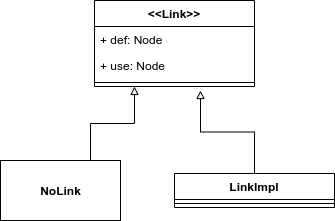
\includegraphics [scale=0.75] {nolink}
	\caption{Иерархия Link с NoLink в качестве объекта по-умолчанию}
	\label{fig:nolink}
\end{figure}

\FloatBarrier

\subsection{Внедрение зависимостей в Scala}

Особенности Scala позволяют использовать средства языка для построения
компонентно-ориентированных архитектур и внедрения зависимостей. Scala
вместо интерфейсов поддерживает типажи (англ. --- traits) --- набор
методов, используемых для расширения функциональности класса. В отличие
от интерфейсов, типажам позволяется реализация методов. Типажи, если
у них отстутствуют пересекающиеся сигнатуры методов, могут быть скомбинированы
в один конкретный тип данных:

\begin{lstlisting}[language=Scala]
trait A
trait B

class C extends A with B
\end{lstlisting}

Также на типажи могут быть наложены ограничения --- можно задать тип,
сигнатурами которого должен обладать класс, с которым комбинируется типаж:

\begin{lstlisting}[language=Scala]
trait A

// Типаж B комбинируется только с классом, имеющим черты типажа A
trait B { this: A => }

// Программа успешно скомпилируется
class C extends A with B

// Компилятор выдаст ошибку о несопоставимых типах
class D extends B
\end{lstlisting}

При этом в типаже B становится возможным использовать переменные и методы,
определенные в типаже A.

Определение набора типажей, взаимных ограничений на их комбинацию,
и составление в один объект, возможно, определяющий цепочку действий,
составленных из методов типажей, в среде Scala-разработчиков имеет название
<<Cake pattern>> (по аналогии с процессом приготовления пирога) \cite{cakepattern}.

В коде компилятора шаблон используется для составления компилятора из
множества проходов --- входных, оптимизирующих, выходных:

\begin{lstlisting}[language=Scala]
class Compiler(folder: String) extends Env with PayloadParser with Sandbox with IRBuilder with Optimizer with CodeGenerator with IndexBuilder {

def configure(): Unit = {
    Env.projectFolder = folder

    Env.useTailCallElimination = payload.compiler.flags.`tail-call-elimination`
    Env.useCommonRecursionMemoization = payload.compiler.flags.`common-recursion-memoization`
    Env.useFibonacciRecursionElimination = payload.compiler.flags.`fibonacci-elimination`
}

def createOutDirectory(): Unit = {
    new File(Env.outFolder).mkdir()
}

configure()

buildIR()
optimize()

createOutDirectory()

buildIndex()
generate()

}
\end{lstlisting}

\section{Описание методов интегрированной среды визуального программирования}\label{sec:ch3/sect3}

App --- корневой компонент приложения, содержащий другие компоненты. Члены компонента представлены в таблице \ref{tab:class1}

\begin{longtable} {| p{8.3cm} | p{8.35cm}l |}
	\caption{Члены компонента App}
	\label{tab:class1}\\
	\hline
	\centering Наименование &  \centering Описание & \\
	\hline
	\endfirsthead
	\caption*{Продолжение таблицы \ref{tab:class1}}\\
	\hline
	\endhead
	\hline
	\endfoot
	loadProject() & отправляет HTTP-запрос на загрузку данных о проекте & \\
	\hline
	saveProject() & отправляет HTTP-запрос на сохранение данных о проекте & \\
\end{longtable}

NavBar --- навигационная панель, содержащая управляющие элементы для перехода между экранами. Члены компонента представлены в таблице \ref{tab:class2}

\begin{longtable} {| p{8.3cm} | p{8.35cm}l |}
	\caption{Члены компонента NavBar}
	\label{tab:class2}\\
	\hline
	\centering Наименование &  \centering Описание & \\
	\hline
	\endfirsthead
	\caption*{Продолжение таблицы \ref{tab:class2}}\\
	\hline
	\endhead
	\hline
	\endfoot
	shutDownSession() & отправляет HTTP-запрос на выключение сервера среды и закрывает вкладку браузера & \\
	\hline
	buildProject() & отправляет HTTP-запрос на сборку проекта & \\
	\hline
	runProject() & отправляет HTTP-запрос на сборку проекта и открывает вкладку с собранным приложением & \\
	\hline
	hotkeys(e: KeyboardEvent) & порождает события по нажатию комбинации клавиш & \\
\end{longtable}

Settings --- экран настроек проекта. Члены компонента представлены в таблице \ref{tab:class3}

\begin{longtable} {| p{8.3cm} | p{8.35cm}l |}
	\caption{Члены компонента Settings}
	\label{tab:class3}\\
	\hline
	\centering Наименование &  \centering Описание & \\
	\hline
	\endfirsthead
	\caption*{Продолжение таблицы \ref{tab:class3}}\\
	\hline
	\endhead
	\hline
	\endfoot
	saveSettings() & сохраняет выбранные настройки проекта & \\
\end{longtable}

ModelProperties --- содержимое панели <<Свойства>> модуля <<Модель>>. Члены компонента представлены в таблице \ref{tab:class4}

\begin{longtable} {| p{8.3cm} | p{8.35cm}l |}
	\caption{Члены компонента ModelProperties}
	\label{tab:class4}\\
	\hline
	\centering Наименование &  \centering Описание & \\
	\hline
	\endfirsthead
	\caption*{Продолжение таблицы \ref{tab:class4}}\\
	\hline
	\endhead
	\hline
	\endfoot
	addVariant() & добавляет вариант в тип-сумму & \\
	\hline
	deleteVariant(i) & удаляет i-й вариант типа-суммы & \\
\end{longtable}

ModelWorkspace --- рабочая область модуля <<Модель>>. Члены компонента представлены в таблице \ref{tab:class5}

\begin{longtable} {| p{8.3cm} | p{8.35cm}l |}
	\caption{Члены компонента ModelWorkspace}
	\label{tab:class5}\\
	\hline
	\centering Наименование &  \centering Описание & \\
	\hline
	\endfirsthead
	\caption*{Продолжение таблицы \ref{tab:class5}}\\
	\hline
	\endhead
	\hline
	\endfoot
	addType(name: string, e: DragEvent) & добавляет тип в рабочую область & \\
	\hline
	setCurrentType(t) & устанавливает выделенный тип в рабочей области & \\
\end{longtable}

Alias --- представление типа-псевдонима на рабочей области модуля <<Модель>>. Члены компонента представлены в таблице \ref{tab:class6}

\begin{longtable} {| p{8.3cm} | p{8.35cm}l |}
	\caption{Члены компонента Alias}
	\label{tab:class6}\\
	\hline
	\centering Наименование &  \centering Описание & \\
	\hline
	\endfirsthead
	\caption*{Продолжение таблицы \ref{tab:class6}}\\
	\hline
	\endhead
	\hline
	\endfoot
	setCurrentRefinedType() & обновляет данные типа для представления на панели свойств & \\
\end{longtable}

Variant --- представление типа-суммы на рабочей области модуля <<Модель>>. Члены компонента представлены в таблице \ref{tab:class7}

\begin{longtable} {| p{8.3cm} | p{8.35cm}l |}
	\caption{Члены компонента Variant}
	\label{tab:class7}\\
	\hline
	\centering Наименование &  \centering Описание & \\
	\hline
	\endfirsthead
	\caption*{Продолжение таблицы \ref{tab:class7}}\\
	\hline
	\endhead
	\hline
	\endfoot
	setCurrentRefinedType() & обновляет данные типа для представления на панели свойств & \\
\end{longtable}

ViewWorkspace --- рабочая область модуля <<Представление>>. Члены компонента представлены в таблице \ref{tab:class8}

\begin{longtable} {| p{8.3cm} | p{8.35cm}l |}
	\caption{Члены компонента ViewWorkspace}
	\label{tab:class8}\\
	\hline
	\centering Наименование &  \centering Описание & \\
	\hline
	\endfirsthead
	\caption*{Продолжение таблицы \ref{tab:class8}}\\
	\hline
	\endhead
	\hline
	\endfoot
	addWidget(name: string, e: DragEvent) & добавляет виджет в рабочую область & \\
	\hline
	setCurrentWidget(w) & устанавливает выделенный виджет в рабочей области & \\
\end{longtable}

Pane --- представление главной панели приложения на рабочей области модуля <<Представление>>. Члены компонента представлены в таблице \ref{tab:class9}

\begin{longtable} {| p{8.3cm} | p{8.35cm}l |}
	\caption{Члены компонента Pane}
	\label{tab:class9}\\
	\hline
	\centering Наименование &  \centering Описание & \\
	\hline
	\endfirsthead
	\caption*{Продолжение таблицы \ref{tab:class9}}\\
	\hline
	\endhead
	\hline
	\endfoot
	setCurrentRefinedWidget() & обновляет данные виджета для представления на панели свойств & \\
\end{longtable}

Button --- представление виджета <<Кнопка>> на рабочей области модуля <<Представление>>. Члены компонента представлены в таблице \ref{tab:class10}

\begin{longtable} {| p{8.3cm} | p{8.35cm}l |}
	\caption{Члены компонента Button}
	\label{tab:class10}\\
	\hline
	\centering Наименование &  \centering Описание & \\
	\hline
	\endfirsthead
	\caption*{Продолжение таблицы \ref{tab:class10}}\\
	\hline
	\endhead
	\hline
	\endfoot
	setCurrentRefinedWidget() & обновляет данные виджета для представления на панели свойств & \\
\end{longtable}

Label --- представление виджета <<Метка>> на рабочей области модуля <<Представление>>. Члены компонента представлены в таблице \ref{tab:class11}

\begin{longtable} {| p{8.3cm} | p{8.35cm}l |}
	\caption{Члены компонента Label}
	\label{tab:class11}\\
	\hline
	\centering Наименование &  \centering Описание & \\
	\hline
	\endfirsthead
	\caption*{Продолжение таблицы \ref{tab:class11}}\\
	\hline
	\endhead
	\hline
	\endfoot
	setCurrentRefinedWidget() & обновляет данные виджета для представления на панели свойств & \\
\end{longtable}

TextBox --- представление виджета <<Поле ввода>> на рабочей области модуля <<Представление>>. Члены компонента представлены в таблице \ref{tab:class12}

\begin{longtable} {| p{8.3cm} | p{8.35cm}l |}
	\caption{Члены компонента TextBox}
	\label{tab:class12}\\
	\hline
	\centering Наименование &  \centering Описание & \\
	\hline
	\endfirsthead
	\caption*{Продолжение таблицы \ref{tab:class12}}\\
	\hline
	\endhead
	\hline
	\endfoot
	setCurrentRefinedWidget() & обновляет данные виджета для представления на панели свойств & \\
\end{longtable}

UpdateWorkspace --- рабочая область модуля <<Обновление>>. Члены компонента представлены в таблице \ref{tab:class13}

\begin{longtable} {| p{8.3cm} | p{8.35cm}l |}
	\caption{Члены компонента UpdateWorkspace}
	\label{tab:class13}\\
	\hline
	\centering Наименование &  \centering Описание & \\
	\hline
	\endfirsthead
	\caption*{Продолжение таблицы \ref{tab:class13}}\\
	\hline
	\endhead
	\hline
	\endfoot
	deleteItem(i) & удаляет i-й элемент в списке объектов рабочей области & \\
\end{longtable}

Connections --- компонент управления связями между объектами модуля <<Обновление>>. Члены компонента представлены в таблице \ref{tab:class14}

\begin{longtable} {| p{8.3cm} | p{8.35cm}l |}
	\caption{Члены компонента Connections}
	\label{tab:class14}\\
	\hline
	\centering Наименование &  \centering Описание & \\
	\hline
	\endfirsthead
	\caption*{Продолжение таблицы \ref{tab:class14}}\\
	\hline
	\endhead
	\hline
	\endfoot
	setSource(s) & устанавливает текущее начало связи между объектами & \\
	\hline
	addConnection(d) & создает связь между установленным началом связи и объектом d & \\
\end{longtable}

\section{Описание методов оптимизирующего компилятора}\label{sec:ch3/sect4}

App --- точка входа, предоставляющая интерфейс командной строки для работы с компилятором. Члены класса представлены в таблице \ref{tab:class15}

\begin{longtable} {| p{8.3cm} | p{8.35cm}l |}
	\caption{Члены класса App}
	\label{tab:class15}\\
	\hline
	\centering Наименование &  \centering Описание & \\
	\hline
	\endfirsthead
	\caption*{Продолжение таблицы \ref{tab:class15}}\\
	\hline
	\endhead
	\hline
	\endfoot
	run(args: List[String]): Unit & выполняет указанную команду в зависимости от переданных аргументов & \\
\end{longtable}

Actions --- набор действий, выполняемых интерпретатором командной строки. Члены класса представлены в таблице \ref{tab:class16}

\begin{longtable} {| p{8.3cm} | p{8.35cm}l |}
	\caption{Члены класса Actions}
	\label{tab:class16}\\
	\hline
	\centering Наименование &  \centering Описание & \\
	\hline
	\endfirsthead
	\caption*{Продолжение таблицы \ref{tab:class16}}\\
	\hline
	\endhead
	\hline
	\endfoot
	launchIde(folder: String): Unit & запускает среду для проекта в каталоге folder & \\
	\hline
	buildProject(folder: String): Unit & собирает проект в каталоге folder & \\
\end{longtable}

FlovverServer --- сервер интегрированной среды разработки. Члены класса представлены в таблице \ref{tab:class17}

\begin{longtable} {| p{8.3cm} | p{8.35cm}l |}
	\caption{Члены класса FlovverServer}
	\label{tab:class17}\\
	\hline
	\centering Наименование &  \centering Описание & \\
	\hline
	\endfirsthead
	\caption*{Продолжение таблицы \ref{tab:class17}}\\
	\hline
	\endhead
	\hline
	\endfoot
	run(folder: String): Unit & запускает сервер для проекта в каталоге folder & \\
\end{longtable}

Widgets --- предоставляемый набор виджетов. Члены класса представлены в таблице \ref{tab:class18}

\begin{longtable} {| p{8.3cm} | p{8.35cm}l |}
	\caption{Члены класса Widgets}
	\label{tab:class18}\\
	\hline
	\centering Наименование &  \centering Описание & \\
	\hline
	\endfirsthead
	\caption*{Продолжение таблицы \ref{tab:class18}}\\
	\hline
	\endhead
	\hline
	\endfoot
	button(id, caption, x, y, width, height, onclick): Widget & создает виджет типа <<Кнопка>> & \\
	\hline
	textBox(id, caption, x, y, width, height, onclick): Widget & создает виджет типа <<Текстовая форма>> & \\
	\hline
	label(id, caption, x, y, width, height, onclick): Widget & создает виджет типа <<Метка>> & \\
\end{longtable}

CodeGenerator --- генератор JavaScript-кода. Члены класса представлены в таблице \ref{tab:class19}

\begin{longtable} {| p{8.3cm} | p{8.35cm}l |}
	\caption{Члены класса CodeGenerator}
	\label{tab:class19}\\
	\hline
	\centering Наименование &  \centering Описание & \\
	\hline
	\endfirsthead
	\caption*{Продолжение таблицы \ref{tab:class19}}\\
	\hline
	\endhead
	\hline
	\endfoot
	topSort(): Unit & топологически сортирует внутреннее представление & \\
	\hline
	generate() & генерирует JavaScript-код программы & \\
\end{longtable}

IRBuilder --- генератор внутреннего представления. Члены класса представлены в таблице \ref{tab:class20}

\begin{longtable} {| p{8.3cm} | p{8.35cm}l |}
	\caption{Члены класса IRBuilder}
	\label{tab:class20}\\
	\hline
	\centering Наименование &  \centering Описание & \\
	\hline
	\endfirsthead
	\caption*{Продолжение таблицы \ref{tab:class20}}\\
	\hline
	\endhead
	\hline
	\endfoot
	buildIR(): Unit & строит внутреннее представление по разобранным данным проекта & \\
\end{longtable}

PayloadParser --- парсер данных проекта. Члены класса представлены в таблице \ref{tab:class21}

\begin{longtable} {| p{8.3cm} | p{8.35cm}l |}
	\caption{Члены класса PayloadParser}
	\label{tab:class21}\\
	\hline
	\centering Наименование &  \centering Описание & \\
	\hline
	\endfirsthead
	\caption*{Продолжение таблицы \ref{tab:class21}}\\
	\hline
	\endhead
	\hline
	\endfoot
	parse[A: AsJsonInput](source: A): Payload & разбирает данные и переводит в программное представление & \\
\end{longtable}

Sandbox --- окружение для работы с внутренним представлением. Члены класса представлены в таблице \ref{tab:class22}

\begin{longtable} {| p{8.3cm} | p{8.35cm}l |}
	\caption{Члены класса Sandbox}
	\label{tab:class22}\\
	\hline
	\centering Наименование &  \centering Описание & \\
	\hline
	\endfirsthead
	\caption*{Продолжение таблицы \ref{tab:class21}}\\
	\hline
	\endhead
	\hline
	\endfoot
	addNode[N <: Node](n: N): N & добавляет вершину во внутреннее представление & \\
	\hline
	collect[T : ClassTag]: Iterator[T] & собирает все вершины заданного типа & \\
	\hline
	use(defNode, useNode, useArg) & задает внешнюю связь между вершинами & \\
	\hline
	output(defNode, useNode) & задает связь между вершиной и выходом определения функции & \\
	\hline
	input(defNode, parameter, useNode, useArg) & задает связь между входом определения функции и вершиной & \\
\end{longtable}

Optimizer --- оптимизатор компилятора. Члены класса представлены в таблице \ref{tab:class23}

\begin{longtable} {| p{8.3cm} | p{8.35cm}l |}
	\caption{Члены класса Optimizer}
	\label{tab:class23}\\
	\hline
	\centering Наименование &  \centering Описание & \\
	\hline
	\endfirsthead
	\caption*{Продолжение таблицы \ref{tab:class23}}\\
	\hline
	\endhead
	\hline
	\endfoot
	optimize(): Unit & запускает оптимизирующие проходы & \\
\end{longtable}

TailCallElimination --- оптимизирующий проход устранения хвостовой рекурсии. Члены класса представлены в таблице \ref{tab:class24}

\begin{longtable} {| p{8.3cm} | p{8.35cm}l |}
	\caption{Члены класса TailCallElimination}
	\label{tab:class24}\\
	\hline
	\centering Наименование &  \centering Описание & \\
	\hline
	\endfirsthead
	\caption*{Продолжение таблицы \ref{tab:class24}}\\
	\hline
	\endhead
	\hline
	\endfoot
	markTailCalls(): Unit & помечает удовлетворяющие определения функций как хвосто-рекурсивные & \\
\end{longtable}

IndexBuilder --- генератор HTML-кода приложения на основе данных о представлении. Члены класса представлены в таблице \ref{tab:class25}

\begin{longtable} {| p{8.3cm} | p{8.35cm}l |}
	\caption{Члены класса IndexBuilder}
	\label{tab:class25}\\
	\hline
	\centering Наименование &  \centering Описание & \\
	\hline
	\endfirsthead
	\caption*{Продолжение таблицы \ref{tab:class25}}\\
	\hline
	\endhead
	\hline
	\endfoot
	buildIndex(): Unit & строит <<index.html>> для заданного проекта & \\
\end{longtable}

